%----------------------------------------------------
% Setup Beamer
%----------------------------------------------------
\documentclass[hyperref={colorlinks=true}]{beamer}

%----------------------------------------------------
% Packages to use
%----------------------------------------------------
\input{../packages.sty}

%----------------------------------------------------
% Setup Theme
%----------------------------------------------------
\input{../theme.sty}

%----------------------------------------------------
% Table of Contents at each section transition
%----------------------------------------------------

\AtBeginSection[]
{
   \begin{frame}
       \frametitle{Outline}
       \setcounter{tocdepth}{2}
       \tableofcontents[currentsection]
   \end{frame}
}

%----------------------------------------------------
% Colors
%----------------------------------------------------
\input{../mycolors.sty}

%----------------------------------------------------
% Style, formatting, and new commands
%----------------------------------------------------
\newcommand{\CourseYear}   {2025}
\newcommand{\CanvasURL}    {https://canvas.uchicago.edu/courses/66016}
\newcommand{\CanvasLink}   {\href{\CanvasURL}{\CanvasURL}}
\newcommand{\GitHubURL}    {https://github.com/UChicagoPhysics/PHYS250}
\newcommand{\GitHubLink}   {\href{\GitHubURL}{\GitHubURL}}
\newcommand{\PlatformURL}  {https://binderhub.pile.uchicago.edu/}
\newcommand{\PlatformLink} {\href{\PlatformURL}{\PlatformURL}}
\newcommand{\PiazzaURL}    {https://canvas.uchicago.edu/courses/66016/discussion\_topics}
\newcommand{\PiazzaLink}   {\href{\PiazzaURL}{\PiazzaURL}}
\input{../newcommands.sty}

%----------------------------------------------------
% Set paths for plots and images
%----------------------------------------------------
\input{../paths.sty}


%-----------------------------------------------------------------------------------------
% Title: [Column]{Title}
%-----------------------------------------------------------------------------------------
\title[PHYS 250 (Autumn 2025) TODAY -- Lecture 1]{Random numbers, their generation, and their peculiarities}

%-----------------------------------------------------------------------------------------
% SubTitle: [Column]{Subtitle}
%-----------------------------------------------------------------------------------------
\subtitle{PHYS 250 (Autumn 2025) -- Lecture 2}

%-----------------------------------------------------------------------------------------
% Author: [SubAuthor]{Author}
%-----------------------------------------------------------------------------------------
\author[D.W.~Miller]{David Miller}

%----------------------------------------------------
% Institute: [SubInst]{Institute}
%----------------------------------------------------
\institute[EFI, Chicago] 
{
  Department of Physics and the Enrico Fermi Institute\\
  University of Chicago
}

%----------------------------------------------------
% Institute: [SubInst]{Institute}
%----------------------------------------------------
\date[October 3, 2024]{October 3, 2024}

\subject{PHYS 250 Lecture}

\begin{document}

%==========================================================================================
% TITLE PAGE
%==========================================================================================

{
\begin{frame}
  \titlepage
\end{frame}
}

%==========================================================================================
\section[Quick \git/\github tutorial]{Quick \git/\github tutorial}
%==========================================================================================

%-----------------------------------------------------------------------------------------
\subsection[Basics of \git]{Basics of \git}
%-----------------------------------------------------------------------------------------

\begin{frame}%[shrink=10]
  \frametitle{Version control reminders}
  
  \begin{center}
    \includegraphics[width=0.25\columnwidth]{/Users/fizisist/Pictures/Random/Git-Logo-2Color.png}
    \includegraphics[width=0.25\columnwidth]{/Users/fizisist/Pictures/Random/GitHub_Logo.png}
  \end{center}

  We will be using these tools for the course. There are \alertbf{many} awesome tutorials out there, and here are a few of my favorite bookmarks:
  
  \begin{itemize}
    \item \href{https://guides.github.com/activities/hello-world/}{``Hello World'' from \github}
    \item \href{https://product.hubspot.com/blog/git-and-github-tutorial-for-beginners}{An Intro to Git and GitHub for Beginners (Tutorial)}
    \item \href{http://marklodato.github.io/visual-git-guide/index-en.html}{A Visual Git Reference}
    \item \href{https://medium.com/@abhishekj/an-intro-to-git-and-github-1a0e2c7e3a2f}{An Intro to Git and GitHub}
  \end{itemize}

  A basic summary of the concept of \git, in my words, is:
  
  \begin{ucblock}{}
    \centering \textbf{\git takes a snapshot of the entire ``project'' and saves it, kind of like running Time Machine (or any disk backup) on your entire hard drive every time.}
  \end{ucblock}


\end{frame}

%-----------------------------------------------------------------------------------------

\begin{frame}%[shrink=10]
  \frametitle{\git concept in pictures}
  
  \begin{center}
    \includegraphics[width=0.75\columnwidth]{GitFlow.png}\\
    \includegraphics[width=0.65\columnwidth]{GitCheckins.png}
  \end{center}
  
  
\end{frame}

%-----------------------------------------------------------------------------------------
\subsection[\git workflow]{\git workflow}
%-----------------------------------------------------------------------------------------

\begin{frame}%[shrink=10]
  \frametitle{What does a \git work flow look like?}
  
  \begin{center}
    \includegraphics<1>[width=0.85\columnwidth]{GitHubWorkflow.png}%
    \includegraphics<2>[width=0.90\columnwidth]{GitHubWorkflow-commands.png}%
  \end{center}
  
  
\end{frame}

%-----------------------------------------------------------------------------------------

\begin{frame}%[shrink=10]
  \frametitle{What does a \git work flow look like?}
  
  \begin{columns}
    
    \column{0.6\textwidth}
    
    The five commands you use the most are:
    
      \begin{itemize}
        \item \texttt{git add \textit{files}}: copies \texttt{\textit{files}} (at their current state) to the stage.
        \item \texttt{git commit -m "MESSAGE"}: saves a snapshot of the stage as a commit.
        \item \texttt{git reset \textit{files}}: copies \texttt{\textit{files}} from the latest commit to the stage. 
        \begin{itemize}
          \item Use this command to ``undo'' a \texttt{git add \textit{files}}. You can also git reset to unstage everything.
        \end{itemize}
        \item \texttt{git checkout \textit{files}}:  copies \texttt{\textit{files}} from the stage to the working directory. Use this to throw away local changes.
        \item \texttt{git push}: send everything in your local repository back to the master
      \end{itemize}
    
    \column{0.4\textwidth}
    
      \begin{center}
        \includegraphics[width=0.95\columnwidth]{GitStages.png}\\ 
        \vfill
        \includegraphics[width=1.25\columnwidth]{GitBasicUsage.png}
      \end{center}
    
  \end{columns}
  
  
\end{frame}

%-----------------------------------------------------------------------------------------

\begin{frame}%[shrink=10]
  \frametitle{\git workflow example: edit \texttt{HelloGaussian.py}}
  
  \begin{center}
    \foreach \n in {1,...,17}%
      {\includegraphics<\n>[width=0.95\columnwidth]{GitWorkflow-Example-\n.png}}
  \end{center}
    
\end{frame}

%-----------------------------------------------------------------------------------------
\subsection[Our usage of \git and \github resources]{Our usage of \git and \github resources}
%-----------------------------------------------------------------------------------------

\begin{frame}%[shrink=10]
  \frametitle{PHYS 250 \github}
  \framesubtitle{\url{https://github.com/UChicagoPhysics/PHYS250}}
  
  Course materials are hosted in the \github \texttt{UChicagoPhysics} repository
  
  \begin{center}
    \includegraphics[width=0.85\textwidth]{../Lecture1/PHYS250-GitHub.png}
  \end{center}

  \vspace{-0.5cm}

  \begin{itemize}
    \item Slides (e.g. \textit{these!}), syllabi, learning goals, and code examples
    \item Stable versions will be cross-posted to \href{\CanvasURL}{Canvas} as well.
    \item Homework submission will be done via \github (\textit{instructions to come})
  \end{itemize}
  
  
\end{frame}

%==========================================================================================
\section[Plan for homework]{Plan for homework}
%==========================================================================================

%-----------------------------------------------------------------------------------------
\subsection[Using \github Classroom]{Using \github Classroom}
%-----------------------------------------------------------------------------------------


\begin{frame}%[shrink=10]
  \frametitle{\github Classroom: assignments (I)}
  
  As mentioned on Tuesday, we will be using \github for distribution, assessment, and collection of assignments. 
  
  \begin{center}
    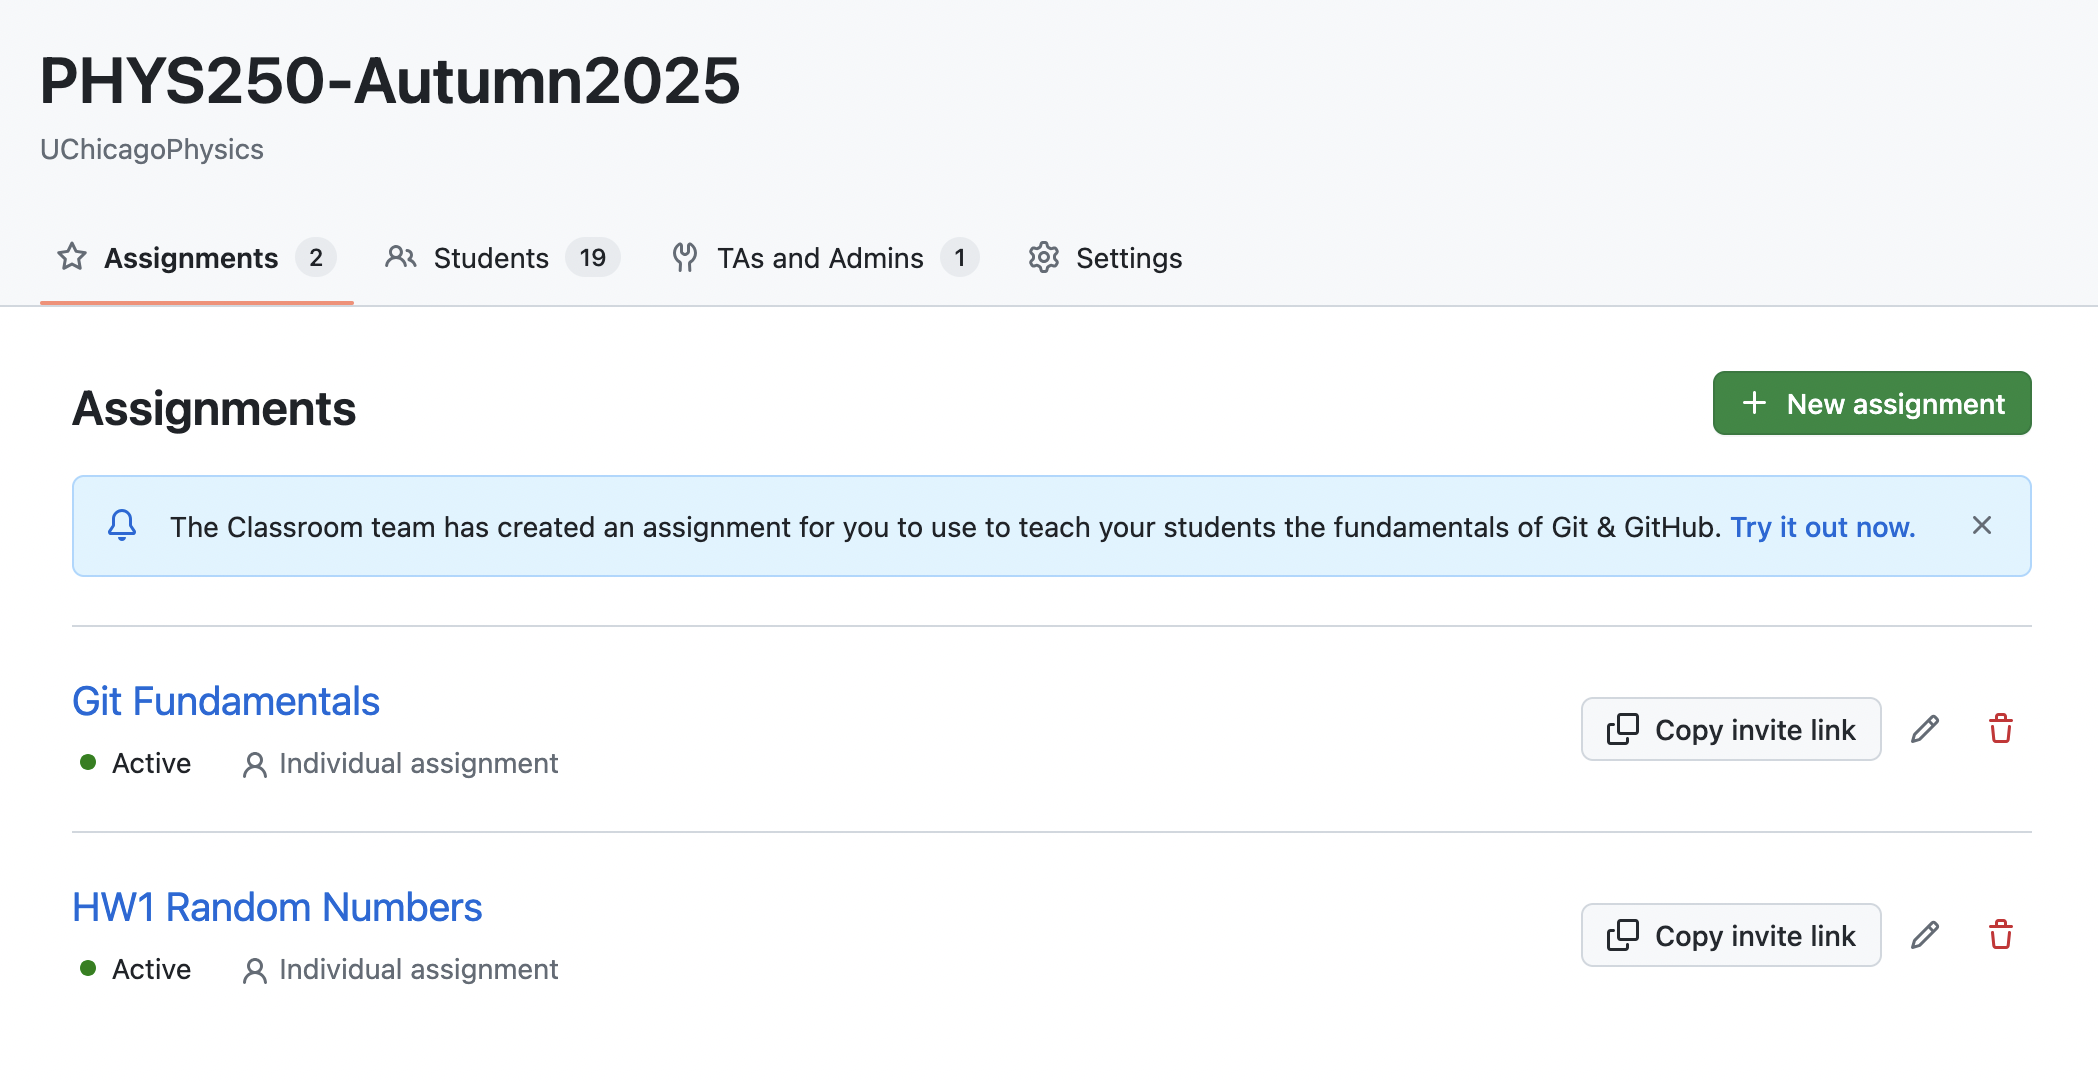
\includegraphics[width=0.65\textwidth]{GitHubClassroom-Assignment1.png}
  \end{center}
  
  %\vspace{-1cm}
  
  \centering HW1: \url{https://classroom.github.com/a/6VzTjkBn} \\
  \centering Git Practice: \url{https://classroom.github.com/a/898iwBYs}

\end{frame}

%-----------------------------------------------------------------------------------------

\begin{frame}%[shrink=10]
  \frametitle{\github Classroom: assignments (II)}
  
  \begin{itemize}
    \item You will receive a link to the assignment
    \begin{itemize}
      \item \url{https://classroom.github.com/a/6VzTjkBn}
    \end{itemize}
    \item This provides your own unique respiratory based on a starter repository with examples and info that you might find useful for the assignment. 
    \item The deadline will be \textbf{Thursday at 2pm}, at which time \github Classroom will save the latest commit from each repository as a submission. 
    \item Submission commits are viewable \alertbf{only to me and the TAs} on the assignment page. 
    \item We can then make comments and grades directly on your submission.
  \end{itemize}
  
  %For a tutorial about how this works, see this 3.5 min video:

  %\centering \url{https://youtu.be/rTsfBAV7sOo}

\end{frame}

%==========================================================================================
\section[Physics]{Physics}
%==========================================================================================

%-----------------------------------------------------------------------------------------
\subsection[Random numbers: Introduction and motivation]{Random numbers: Introduction and motivation}
%-----------------------------------------------------------------------------------------

\begin{frame}%[shrink=10]
  \frametitle{Random numbers}
  
  Random numbers may seem innocuous, but they underlie nearly everything you do electronically, rely on for security, or employ in the context of simulations and evaluation of models.
  
  \begin{itemize}
    \item \bluebf{cryptography}
    \item \bluebf{computer simulation}
    \begin{itemize}
      \item  most well-known of which is named after gambling town, \alertbf{Monte Carlo}
    \end{itemize}
    \item \bluebf{sampling}
  \end{itemize}

  As such, their use, their control, and the evaluation of just how random they are, are of \alertbf{paramount importance for computational physics.}

\end{frame}

%-----------------------------------------------------------------------------------------

\begin{frame}%[shrink=10]
  \frametitle{And you thought lava lamps were a thing of the past}
  
  \begin{figure}
    \centering
    \includegraphics[width=0.85\textwidth]{LavaLamps.jpg}
  \end{figure}

  Cryptography relies on the ability to generate random numbers that are both unpredictable and  secret. But \alertbf{random} is a very malleable term. 

\end{frame}

%-----------------------------------------------------------------------------------------
\subsection[Types of random numbers]{Types of random numbers}
%-----------------------------------------------------------------------------------------

\begin{frame}%[shrink=10]
  \frametitle{True vs. Pseudo: it's more than semantics}
  
  The computers of today are, by design and by implementation, \bluebf{\textit{deterministic}}.  That means that an \alertbf{algorithm cannot}, on its own and without input from an external source, provide a stream of 100\% uncorrelated random sequences. Hence the division:
  
  \begin{itemize}
    \item \textbf{TRNGs:} \bluebf{True} random number generators
    \begin{itemize}
      \item generally use some physical process that is unpredictable, but often slow and requires specialized hardware
      \item possibly combined with some compensation mechanism that might remove any bias in the process
      \item examples include: lava lamps, quantum processes, radioactive decays, thermal noise
    \end{itemize}
    \item \textbf{PRNGs:} \bluebf{Pseudo-}random number generators
    \begin{itemize}
      \item based on algorithms and, therefore, not truly \textit{random}
      \item do not require special hardware and therefore are very portable and fast
      \item can be reproduced given initial conditions
    \end{itemize}
  \end{itemize}
  
  \centering \textbf{We will, perhaps obviously, focus on PRNGs.} 
  
  \textit{(but if you want to build a wall of lava lamps in KPTC, I will cheer you on)}

\end{frame}

%-----------------------------------------------------------------------------------------

\begin{frame}%[shrink=10]
  \frametitle{Pseudo-random number generators (PRNGs)}
  
  The idea behind an algorithmic PRNG is to generate a sequence of numbers, $x_1, x_2, x_3 ...$ using a recurrence of the form
  %
  \begin{equation}
    x_i = f(x_{i-1}, x_{i-2}, ..., x_{i-n}),
  \end{equation}

  where $n$ initial numbers (``seeds'') are needed to begin the recurrence. The magic lies in the function, $f$, used, and the resulting \textit{uniformity} and \textit{correlation length} across some sequence of numbers. 
  
  Linear congruential generators (LCGs) are one of the oldest PRNGs and have the form
  %
  \begin{equation}
    x_{i+1} = (a x_i + c) \mod m
  \end{equation}

  IBM mainframes in the 60s had $a = 65539$, $c = 0$, and $m = 2^{31}$. This leads to
  %
  \begin{equation}
    x_{i+2} = 6 x_{i+1} - 9x_i
  \end{equation}

  which, maybe you can tell, isn't great. 

\end{frame}

%-----------------------------------------------------------------------------------------

\begin{frame}[fragile]%[shrink=10]
  \frametitle{Python random number generator: Mersenne Twister}
  
  Python has a built-in (\texttt{stdlib}) RNG that can be accessed with:
  
  \begin{ucpythonblock}{}
import random as rng
rng.random()  
  \end{ucpythonblock}

  \texttt{numpy} has an even more developed set of tools with \texttt{numpy.random}. 
  
  \begin{ucpythonblock}{}
from numpy import random as rng
rng.random()  
  \end{ucpythonblock}  

  Both of these use the \href{https://en.wikipedia.org/wiki/Mersenne_Twister}{Mersenne Twister algorithm}, developed in 1997 by Matsumoto and Nishimura; is a version of a generalized feedback shift register PRNG. The name due to the fact that the period is given by a Mersenne prime (most commonly: $n = 219937$):
  %
  \begin{equation}
    M_n = 2^n - 1, n \in  \mathbb{N}
  \end{equation}

  (In preparing this, I found out that the largest known prime number $2^{77,232,917} - 1$ is a Mersenne prime, found on December 26, 2017.)

\end{frame}

%-----------------------------------------------------------------------------------------
\subsection[Hypothesis testing and random numbers]{Hypothesis testing and random numbers}
%-----------------------------------------------------------------------------------------

\begin{frame}[fragile]%[shrink=10]
  \frametitle{Testing the true ``randomness'' of a RNG}
  
  Tests of RNGs must look for patterns in sequences of given lengths and frequencies and test those possible patterns against the probability that they occurred ``accidentally'' or whether they are happening more often than they \textbf{should}.
  
  \begin{itemize}
    \item[\ra] This brings us to our first example of \bluebf{hypothesis testing}
  \end{itemize}
  
  Big business for RNGs:
  
  \begin{figure}
    \includegraphics[width=\textwidth]{RandomnessTests.png}
  \end{figure}  
  
  See: \url{https://www.random.org}, \url{http://www.cacert.org/}, etc
  
\end{frame}

%-----------------------------------------------------------------------------------------

\begin{frame}[fragile]%[shrink=10]
  \frametitle{Hypothesis testing}
  
  The most common \bluebf{test statistic} is the chi-squared, \chisq
  
  \begin{equation}
    \chisq = \sum_{i=1}^{n} \frac{(O_i - E_i)^2}{E_i} =  N \sum_{i=1}^n \frac{\left(O_i/N - p_i\right)^2}{p_i}
  \end{equation}
where

  \begin{itemize}  
    \item $\chisq$ = Pearson's cumulative test statistic, which asymptotically approaches a $\chisq$.
    \item $O_i$ = the number of observations of type $i$.
    \item $N$ = total number of observations
    \item $p_i$ = the fraction of type $i$ w.r.t. the total ($N$)
    \item $E_i = N p_i$ = the expected (theoretical) count of type $i$
    \item $n$ = the number of cells in the table.
  \end{itemize}
  
  This resembles a normalized sum of squared deviations between observed and theoretical frequencies of occurrence.
  
\end{frame}

%-----------------------------------------------------------------------------------------

\begin{frame}[fragile]%[shrink=10]
  \frametitle{Hypothesis testing in our case}
  
  Instead of testing the \alertbf{randomness} we can test the \bluebf{uniformity} of our RNG using the \chisq and a simple histogram:
  
  \begin{equation}
    \chisq = \sum_{i=1}^{n} \frac{(O_i - E_i)^2}{E_i} =  N \sum_{i=1}^n \frac{\left(O_i/N - p_i\right)^2}{p_i}
  \end{equation}

  In the following, we can think of these quantities as:

  \begin{itemize}  
    \item $O_i$ = the number of times we get a number in some range (i.e. bin $i$ of the histogram)
    \item $N$ = total number of random numbers that we analyze
    \item $p_i$ = the fraction of the total range of the random numbers that each bin $i$ represents
    \item $E_i = N p_i$ = the expected number of times a random number lands in each bin $i$
    \item $n$ = the number of bins in the histogram.
  \end{itemize}
    
\end{frame}



%-----------------------------------------------------------------------------------------

\begin{frame}[fragile]%[shrink=10]
  \frametitle{Testing the uniformity of this PRNG}
  
  A histogram is a graphical representation of a discrete probability distribution. To make a simple histogram, all you need to do is:
  
  \begin{ucpythonblock}{}
# Import the numpy random number generator
from numpy import random as rng

# Import the plotting libraries
import matplotlib.pyplot as plt

# Generate 100 random nums 
# distributed between [0,1)
# (returns a numpy array)
data = rng.random(100) 
 
# Fill a histogram 
plt.hist(data)  
plt.show()
  \end{ucpythonblock}
  
  \pause

  \begin{textblock}{12}(8,-7)
    \includegraphics[width=0.55\textwidth]{RNGHist1.png}
  \end{textblock}  


\end{frame}

%-----------------------------------------------------------------------------------------

\begin{frame}[fragile]%[shrink=10]
  \frametitle{Words of caution regarding hypothesis testing and data sets}
  
  We want to compute a \chisq to see if it's uniform (part of your homework assignment due next Thursday).
  
  However, before going further: be \alertbf{very wary of reliance on any one method} for analyzing a dataset. For example, look at these graphs:
  
  \begin{figure}
    \includegraphics[width=\textwidth]{SameStatsDiffGraphs.pdf}
  \end{figure} 
  
  \pause
  
  As discussed in \href{https://www.autodeskresearch.com/publications/samestats}{this paper}, while different in appearance, \alertbf{each has the same summary statistics to 2 decimal places}:
  
  \begin{itemize}
    \item means: $\overline{x}=54.02, \overline{y}=48.09$
    \item std. deviation: $\sigma_x = 14.52, \sigma_y = 24.79$
    \item Pearson's correlation coefficient: $r = +0.32$
  \end{itemize}


\end{frame}



%%==========================================================================================
%\section[Conclusions]{Conclusions}%==========================================================================================
%
%\begin{frame}%[shrink=1]
%  \frametitle{Conclusions}
%
%  \begin{itemize}
%    \item Something
%  \end{itemize}
%  
%\end{frame}

%==========================================================================================
%==========================================================================================
\end{document}
